\chapter{Graph Theory}
\label{chp:graphTheory} 


\section{Graphs}

Most activities in nature and society can be described using graphs, which offers an intuitive approach that can be analyzed. Railroads, water pipelines, societal relations etc. can all be described using graph theory. In addition, the Internet and other computer networks is formed and evolves according to the laws of random graphs \cite{audestad}. Graphs serves as an analytic tool \cite{audestad}, which in our case makes it possible to investigate whether there are certain graphs that might yield higher security than others. This section will provide background information on how these graphs are created, and highlight the main characteristics which are important for detecting insurable topologies. 

\subsection{Basic graphs}


There are some basic properties of graphs which is important to be familiar with. Figure \ref{fig:generalGraph} depicts the basics of an unweighted graph, meaning the edges are not given any value. In other cases, weighted edges is useful to e.g. reflect capacity constraints such as a link's maximum bandwidth. Other common definition used in the description graphs are described below \cite{audestad}:
\begin{itemize}
\item Edge degree: Number for edges connected with a vertex.
\item Hub: Vertex with high edge degree.
\item Cycle: A chain originating and terminating at the same vertex.
\item Cluster: Subgraph of highly connected vertices.
\item Cluster coefficient: Probability that two vertices that are adjacent to a third vertex are also adjacent.
\item Clique: Subgraph where all vertices are adjacent (cluster coefficient = 1).
\item Small world graph: Graph with small diameter and large cluster coefficient (e.g. the Internet and A-B graphs, described in section \ref{ABgraph}).
\end{itemize}


\begin{figure}[h]
\centering
\begin{tabular}{@{}c@{}}
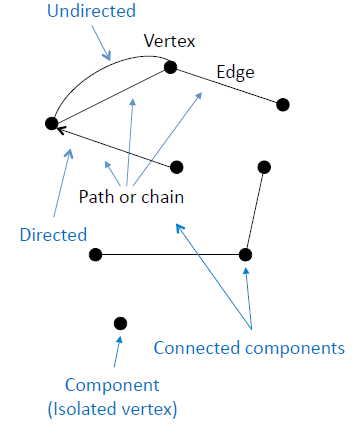
\includegraphics[width=0.4\textwidth]{../Figures/generalGraph.png}
\end{tabular}
\caption{\label{fig:generalGraph} General graph \cite{audestad}.}
\end{figure}


\subsection{Random Graphs}

Regarding cyber-insurance the study of random graphs are of special concern, since we are looking for insurable topologies in computer networks(random graphs). The research on random graphs are fairly new compared with other mathematical discoveries. E-R graphs were first studied in 1959 by Erdös and Rényi, later and probably with more promising results was the graphs studied by Albert-Barabási in 1999 \cite{audestad}. 

\subsubsection{Erdös-Rényi Graphs}
E-R graphs is a network created over a fixed number $n$ of vertices, where each node connects to another of the $n-1$ vertices with a chosen 
probability $p$. The resulting graph will on average contain $n(n-1)p/2 \approx n^{2}p/2$ edges \cite{barabasi}. 
From analyzing the graph, the authors found some interesting properties\cite{barabasi}\cite{audestad}:

\begin{itemize}
\item If $p<n^{-2}$  then there is no edges in the graph. 
\item If $p=c/n$ where c is a constant between $1 < c < log\: n$, the graph will provoke a single large component to grow within the graph.
\item If $p>(ln\: n)/n$ then the graph is completely connected. 
\item If $p = 1/n$ triangles start forming in the graph. 
\end{itemize}

Our goal is to use a graph which models how to Internet and other computer networks are connected. A fully connected E-R graph has a good potential, since the graph will have a short diameter similar to the Internet. However, the edge degree follows a Poisson distribution, which means that the edge degree are peaking around the average value \cite{audestad}. Consequently E-R graphs does not capture the immense clustering coefficient which is present in networks such as the Internet. In other words, E-R graphs are not small world graphs, and another graph structure is needed.



\subsubsection{\label{ABgraph}Albert-Barabási Graphs}
The struckture which is believed to be most accurate regarding modeling the structure of computer networks are A-B graphs. A-B graphs are different from E-R graphs since they are scale-free, meaning that the vertices does not have an constant value throughout the entire graph. The formation of an A-B graph results in multiple hubs with a high edge degree. Albert and Barabási found that the edge degree of each vertex follows a power law distribution; meaning that the probability that the edge degree is $g$ is proportional to $g^{\gamma}$
where $\gamma$ usually is a number between 2 and 3 \cite{audestad}. Consequently there are relatively high probability that a vertex have a very high edge degree. 

A-B graphs can grow and become scale-free if every new vertex is connected to one or more existing vertices with a probability proportional to the edge degree of these vertices \cite{audestad}. The paper \cite{audestad} presents an algorithm creating  A-B graphs and figure \ref{fig:ABgraphcreation} models a possible formation of a graph using the algorithm:


\begin{itemize}
\item A new single vertex is added to the graph.
\item This vertex is connected to exactly two other vertices in the graph.
\item The probability that the new vertex connects to another vertex is dependent on the edge degree of the other vertex, higher edge degree meaning higher probability
\item There is only one edge between two vertices, and the graph does not contain loops.
\end{itemize}


\begin{figure}[h]
\centering
\begin{tabular}{@{}c@{}}
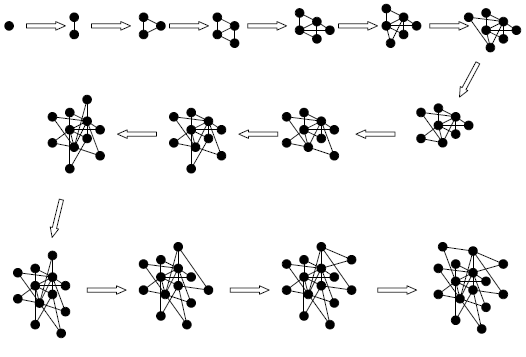
\includegraphics[width=0.8\textwidth]{../Figures/ABgraphcreation.png}
\end{tabular}
\caption{\label{fig:ABgraphcreation} Forming a A-B graph in 15 generations \cite{audestad}.}
\end{figure}

In addition to the high clustering coefficient the research found that these graphs have a fairly small diameter,
 which is noticeable from the graph depicted above. 
 A-B graphs are therefore comparable to the network formation of the Internet and other computer networks. 
The model is therefore a good base in the search for insurable topologies. 

\subsection{Real life graph structures}


The internet, the World Wide Web, neural networks, scientific referencing and co-authorship, stock markets, airline routes, food 
webs, and modular software systems, all tend to evolve in a way similar to that described in the examples 
above \cite{audestad}. This section will provide some real life examples of how complex systems with huge amount of data can be described as network structures having the same characteristics as A-B graphs.

\subparagraph{Stock markets} A research paper from \cite{greekStockMarket} looks at the correlation between stocks in the Greek stock market in year 1997. They compared the daily closing price of stock $i$ at day $t$, and compared the similarity of a pair of stocks $i$ and $j$ a using the correlation coefficient. The idea is that the correlation coefficient between a pair of stocks can be expressed using different distances in a graph structure. A short distance means high correlation and long distance means low correlations between the stocks. Normally this network would be shown as a fully connected graph, which will consist of $\frac{n(n-1)}{2}$ edges, and would be difficult to analyze. However the approach taken in the paper will present a clear understandable graph consisting of $(n-1)$ edges \cite{greekStockMarket}.

The resulting graph is depicted in figure \ref{fig:greekStockMarket}, and show a network consisting of several clusters linked together. Instead of having to analyze a complex system with huge amount of data, this stock market can be analyzed by its topological properties, such as the high clustering coefficient, i.e a star-topology, which will among others point out which stocks have the most influence on others. 


\begin{figure}[h]
\centering
\begin{tabular}{@{}c@{}}
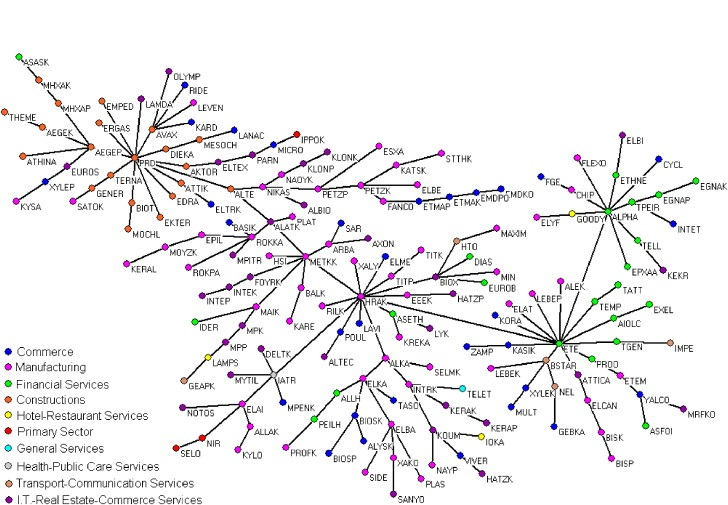
\includegraphics[width=1.0\textwidth]{../Figures/greekStockMarket.jpg}
\end{tabular}
\caption[Caption for LOF]{Network obtained by comparing two stocks correlation coefficient in the Greek stock market (Athens Stock Exchange, ASE) in year 1997. The different colors represent the different sectors of economic activity \cite{greekStockMarket}.
\label{fig:greekStockMarket}}
\end{figure}


\subparagraph{Airline routes}
Another naturally created network which shows characteristics scale-free graphs is the visualization of airline routes. Figure \ref{fig:airlineRouteMap} shows the US route map of the American airline company, SkyWest. The characteristic clustering emerges in the figure, where a majority of the flights departs from either Denver, Chicago or San Francisco. Not surprisingly, these airports are all in the top 7 busiest airports in the US \cite{busiestAirports}, and serves as hubs for many of SkyWest flights. In the airline industry some airports are called hubs, because that's what they are, - a connection point for major parts of the network of flights. The network of flights, as depicted \ref{fig:airlineRouteMap} follows the characteristics for A-B graphs. From the graph, we see that the network are vulnerable against direct attacks, meaning if an low edge degree airport is shut down, there will be little consequence for the rest of the network. However, if one of the hubs is forced to close, it will provoke huge delays through out the whole network of flights, because many of the destinations are interconnected via the hubs. 


\begin{figure}[h]
\centering
\begin{tabular}{@{}c@{}}
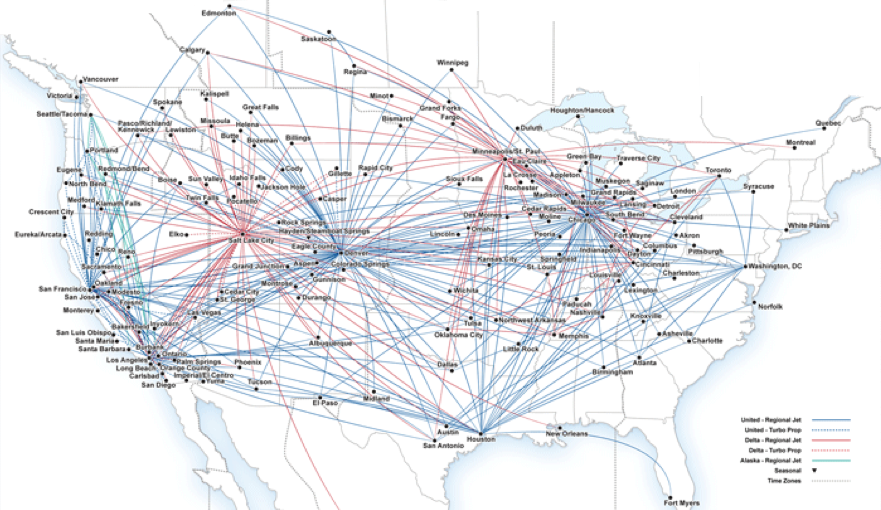
\includegraphics[width=1.0\textwidth]{../Figures/airlineRoutesUSA.png}
\end{tabular}
\caption[Caption for LOF]{SkyWest Airline combined route map \cite{airlineRoutes}.
\label{fig:airlineRouteMap}}
\end{figure}

Similar findings will appear in all the networks mentioned earlier in this section, and everyone will experience serious consequences if a hub in the network is failing. This is important for cyber-insurance because the networks we are analyzing tends to look like and behave according to A-B graphs. For example, transactions between companies could be compared with how the correlation between stocks in a stock market works. Further in this report we will examine how cyber-insurance could benefit from operating in a scale-free graph. 



NOTES!!!
Geek stockmarket graph: http://www.sciencedirect.com/science/article/pii/S037843710700221X



Hvorfor er slike strukturer viktige å forstå for oss? 
Som vi skal se senere oppfører hubene seg i A-B grafene som stjerne-topologier. 
Ved å ha oversikt over sitt eget nettverk vil man kunne identifisere hvor disse stjernene befinner seg, nettopp disse er det viktig at man sikrer for å ungå spredning av virus, samt fungere som en blokkade mot andre trusler e.g. hackers. (TROR DET er viktig at vi prøver å fokusere mot insurable og ikke spredning av virus.)
så noe sånt:
nettopp disse er viktige slik at man lettere kan kalkulere riskioen, og gi insentiver, ved hjelp av cyber insurance, til hubsa for å sikre seg eller no.







